% =============================================================================
% presentation_latex.tex — Beamer presentation
% Zero-Shot Text Classification with Locally-Hosted Large Language Models
% =============================================================================
\documentclass[aspectratio=169,11pt]{beamer}

% ---------- Theme ----------
\usetheme[progressbar=frametitle,
          numbering=fraction,
          sectionpage=progressbar,
          subsectionpage=none]{metropolis}
\setbeamertemplate{navigation symbols}{}

% ---------- Packages ----------
\usepackage[utf8]{inputenc}
\usepackage[T1]{fontenc}
\usepackage{booktabs}
\usepackage{graphicx}
\usepackage{amsmath,amssymb}
\usepackage{xcolor}
\usepackage{array}
\usepackage{listings}

\graphicspath{{experiment/}}

% ---------- Listings setup ----------
\lstdefinelanguage{R}{%
  morekeywords={if,else,for,while,repeat,function,return,in,TRUE,FALSE,
    NULL,NA,Inf,NaN,library,require},
  sensitive=true,
  morecomment=[l]{\#},
  morestring=[b]",
  morestring=[b]',
}
\lstdefinelanguage{Rust}{%
  morekeywords={fn,let,mut,pub,use,mod,struct,enum,impl,trait,return,if,
    else,for,while,loop,match,as,in,ref,move,where,async,await,dyn,unsafe,
    const,static,Self,self,super,crate,true,false,None,Some,Ok,Err,vec},
  sensitive=true,
  morecomment=[l]{//},
  morecomment=[s]{/*}{*/},
  morestring=[b]",
}
\lstset{
  basicstyle=\ttfamily\footnotesize,
  keywordstyle=\color{blue!70!black}\bfseries,
  commentstyle=\color{green!50!black}\itshape,
  stringstyle=\color{red!70!black},
  breaklines=true,
  frame=single,
  numbers=left,
  numberstyle=\tiny\color{gray},
  backgroundcolor=\color{gray!5},
  showstringspaces=false,
}

% ---------- Colors ----------
\definecolor{accent}{HTML}{2E5C8A}
\setbeamercolor{frametitle}{bg=accent}
\setbeamercolor{progress bar}{fg=accent}
\setbeamercolor{alerted text}{fg=accent}

% ---------- Margins ----------
\setbeamersize{text margin left=10mm, text margin right=10mm}

% ---------- Title info ----------
\title{Zero-Shot Text Classification with Locally-Hosted LLMs}
\subtitle{The \texttt{ollama-classifier} Library}
\author{Luigi Palumbo \and Mengting Yu}
\date{July 14, 2026}

% =============================================================================
\begin{document}

\maketitle

% =============================================================================
\section{Motivation}
% =============================================================================

\begin{frame}{The Problem}
  \begin{itemize}
    \item \textbf{Text classification} is pervasive: sentiment analysis,
          product categorization, economic-taxonomy coding
    \item Traditional supervised pipelines demand labeled data, feature
          engineering, and retraining
    \item LLMs enable \textbf{zero-shot} classification via in-context learning
  \end{itemize}
  \vspace{0.4em}
  Yet proprietary cloud APIs:
  \begin{itemize}
    \item incur \textbf{recurring costs}
    \item require \textbf{internet connectivity}
    \item expose \textbf{confidential or regulated data} to third parties
  \end{itemize}
\end{frame}

\begin{frame}{The Opportunity}
  Open-source LLMs (LLaMA, Mistral, Qwen, DeepSeek-R1) + lightweight serving
  (Ollama) run on \textbf{consumer hardware}.

  \vspace{0.6em}
  This creates an opportunity: classification tools that combine the zero-shot
  reasoning of LLMs with the \textbf{privacy}, \textbf{cost-effectiveness}, and
  \textbf{offline capability} of local inference.
\end{frame}

\begin{frame}{\texttt{ollama-classifier} — Three Principles}
  \begin{enumerate}
    \item \textbf{No fine-tuning required.} Classification uses prompting and
          retrieval augmentation.
    \item \textbf{Local and private.} All inference runs on the user's
          hardware — no data leaves the machine.
    \item \textbf{Accompanied by calibrated uncertainty.} Every prediction
          carries a full probability distribution and a confidence score.
  \end{enumerate}
\end{frame}

% =============================================================================
\section{The Library}
% =============================================================================

\begin{frame}{Core API}
  Single backend-agnostic entry point: \texttt{LLMClassifier} over a backend
  such as \texttt{OllamaBackend}.

  \vspace{0.5em}
  \centering
  \small
  \begin{tabular}{lp{7cm}}
    \toprule
    \textbf{Method} & \textbf{Description} \\
    \midrule
    \texttt{classify()} & Multi-call completion scoring: one call per label,
                          exact calibrated probabilities \\
    \texttt{generate()} & Adaptive trie-masked generation: budget-controlled,
                          may be approximate \\
    \texttt{batch\_classify()} / \texttt{batch\_generate()} & Batch variants
                          for many texts \\
    \bottomrule
  \end{tabular}

  \vspace{0.5em}
  \normalsize
  Each method has an \textbf{async} twin (\texttt{aclassify},
  \texttt{agenerate}, \dots).
\end{frame}

\begin{frame}[fragile]{Usage Example — Python}
\begin{lstlisting}[language=Python]
from ollama_classifier import LLMClassifier
from ollama_classifier.backends import OllamaBackend

clf = LLMClassifier(OllamaBackend(model="qwen2.5:3b-instruct"))

choices = {
    "Coffee and coffee substitutes": "Coffee, decaffeinated or not",
    "Tea and other infusions": "Green/black tea",
    "Soft drinks": "Sodas, lemonades, colas, and juices.",
}

result = clf.classify("Instant cafe latte sachet", choices)
# prediction="Coffee...", confidence=0.71, n_calls=4
\end{lstlisting}
\end{frame}

\begin{frame}{Confidence Estimation — \texttt{classify}}
  For each candidate label $y_i$, the backend returns per-token
  log-probabilities of that label's tokens $T_i$ given the prompt.

  \vspace{0.2em}
  \textbf{Label score} (geometric mean of per-token log-probs):
  \[
    s(y_i)=\frac{1}{|T_i|}\sum_{t\in T_i}\log p\!\left(t\mid x,\text{prefix}_t\right)
  \]

  \textbf{Calibrated distribution} (max-subtracted softmax):
  \[
    \text{P}(y_i\mid x)=\frac{\exp\!\left(s(y_i)\right)}{\sum_{j}\exp\!\left(s(y_j)\right)},
    \quad \text{confidence}=\max_i\, \text{P}(y_i\mid x)
  \]

  \vspace{-0.3em}
  \begin{itemize}\setlength{\itemsep}{0.1em}
    \item \textbf{Geometric mean} $\to$ removes length bias;
          \textbf{max-subtracted softmax} $\to$ calibrated distribution
    \item Always exact, one call per label
  \end{itemize}
\end{frame}

\begin{frame}{Confidence Estimation — \texttt{generate}}
  Candidate labels tokenized into a \textbf{prefix trie}; each constrained
  call restricted to trie tokens while returning \texttt{top\_logprobs} of
  every sibling.

  \begin{itemize}
    \item \textbf{Breadth-first search} over clusters of labels sharing a
          scored prefix
    \item Spends between 1 and \texttt{max\_calls} calls
    \item Labels not emitted are still scored via sibling alternatives
    \item \texttt{coverage} $=$ fraction of label's tokens scored;
          \texttt{approximate}$=$\texttt{True} when coverage $< 1$
    \item \texttt{max\_calls}$=1$ $\to$ single fast approximate call;
          \texttt{max\_calls}$=$\texttt{None} $\to$ exact (worst case: one
          call per label)
  \end{itemize}
\end{frame}

\begin{frame}{Backend Differentiation}
  All four backends expose per-token log-probabilities and support both
  strategies.

  \vspace{0.4em}
  \centering
  \footnotesize
  \begin{tabular}{lll}
    \toprule
    \textbf{Backend} & \textbf{Constrained-output mechanism} &
    \textbf{\texttt{classify} scoring path} \\
    \midrule
    Ollama    & JSON Schema enum & Forced constrained generation \\
    vLLM      & \texttt{structured\_outputs.choice} & Echo / prefill \\
    SGLang    & regex alternation & Echo / prefill \\
    llama.cpp & GBNF grammar & Forced constrained generation \\
    \bottomrule
  \end{tabular}

  \vspace{0.5em}
  \normalsize
  vLLM and SGLang score each label as an unconstrained continuation
  (echo/prefill); Ollama and llama.cpp read the \textbf{pre-mask logits}
  (genuine distribution before constraint).
\end{frame}

% =============================================================================
\section{Ecosystem}
% =============================================================================

\begin{frame}{Graphical User Interface}
  \texttt{ollama-classifier-gui} — a companion desktop app (Flet) with five
  tabs:
  \begin{itemize}
    \item \textbf{Settings} — backend, endpoint, model, connection test, API
          key, theme
    \item \textbf{Data Input} — CSV/Excel load, sheet selection, column
          mapping
    \item \textbf{Schema} — labels, Classify/Score method, output format,
          system-prompt override
    \item \textbf{Results} — live progress, Excel export
    \item \textbf{Info} — version and project links
  \end{itemize}

  \vspace{0.3em}
  API keys stored in OS native secure storage (Keychain, Credential Manager,
  libsecret).

  Installs with \texttt{uvx ollama-classifier-gui} or
  \texttt{pip install ollama-classifier-gui}.
\end{frame}

\begin{frame}{Cross-Language Ports}
  \textbf{R: \texttt{rollama-classifier}} — full API port including four
  backends, both strategies, batch twins, and \texttt{classification\_result}
  object. Installs from GitHub:
  \texttt{pak::pak("paluigi/rollama-classifier")}

  \vspace{0.6em}
  \textbf{Rust: \texttt{ollama-classifier-rs}} — mirrors Python API (four
  backends, \texttt{classify}/\texttt{generate}, \texttt{ClassificationResult}
  struct, sync/async/batch). Added with
  \texttt{ollama-classifier-rs = "0.5"} in \texttt{Cargo.toml}.
\end{frame}

\begin{frame}[fragile]{R Port — Example}
\begin{lstlisting}[language=R]
library(rollama)
be <- ollama_backend(model = "llama3.2")
clf <- llm_classifier(be)
res <- classify(clf, "I love this product!",
                c("positive", "negative", "neutral"))
res$prediction
res$confidence
\end{lstlisting}
\end{frame}

\begin{frame}[fragile]{Rust Port — Example}
\begin{lstlisting}[language=Rust]
use ollama_classifier_rs::LLMClassifier;
use ollama_classifier_rs::backends::OllamaBackend;

let be = OllamaBackend::new("llama3.2");
let clf = LLMClassifier::new(be);
let res = clf.classify(
    "I love this product!",
    vec!["positive", "negative", "neutral"],
    None,
)?;
res.prediction
res.confidence
\end{lstlisting}
\end{frame}

% =============================================================================
\section{Application: COICOP Product Classification}
% =============================================================================

\begin{frame}{The Task}
  \textbf{COICOP 2018} — international standard for household expenditure
  categorization: four-level hierarchy, 294 fine-grained subclasses.

  \vspace{0.4em}
  Challenges:
  \begin{itemize}
    \item High linguistic variability across retailers and countries
    \item Strong class imbalance
    \item Textual overlap between semantically similar subclasses
    \item Multilingual coverage needed
  \end{itemize}

  \vspace{0.3em}
  Relevant to \textbf{Consumer Price Index} compilation by National
  Statistical Institutes.
\end{frame}

\begin{frame}{Experimental Setup}
  \begin{itemize}
    \item \textbf{Dataset:} 637 manually labeled products from COICOP
          Division 01.2 (Non-alcoholic beverages), 7 subclasses
    \item \textbf{Baselines:} BART-large-MNLI (NLI zero-shot), scikit-llm
          (\texttt{ZeroShotGPTClassifier})
    \item \textbf{Model:} Qwen2.5 3B-Instruct served by Ollama (shared across
          generative methods)
    \item \textbf{Configurations:} names only, $+$opt-out,
          names$+$descriptions, descriptions$+$opt-out
    \item \textbf{24 variations} total (BART $\times$2, scikit-llm $\times$2,
          classify $\times$4, generate $\times$16)
  \end{itemize}
\end{frame}

% =============================================================================
\section{Results}
% =============================================================================

\begin{frame}{Accuracy — Benchmark (excerpt)}
  \centering
  \footnotesize
  \resizebox{\textwidth}{!}{%
  \begin{tabular}{lccc}
    \toprule
    \textbf{Variation} & \textbf{Acc.\ (\%)} & \textbf{F1 (macro)} &
    \textbf{Time (s)} \\
    \midrule
    BART (names only)         & 40.8 & 0.445 & 444 \\
    BART (names + opt-out)    & 39.4 & 0.454 & 496 \\
    \addlinespace
    Ollama \texttt{classify} (names only)       & \textbf{75.5} & \textbf{0.703} & 2965 \\
    Ollama \texttt{classify} (names + opt-out)  & 74.7 & 0.705 & 3283 \\
    Ollama \texttt{classify} (names + desc.)    & 74.4 & 0.712 & 3007 \\
    Ollama \texttt{classify} (desc. + opt-out)  & 71.3 & 0.709 & 3397 \\
    \addlinespace
    scikit-llm (names only)       & 73.5 & 0.667 & 176 \\
    scikit-llm (names + opt-out)  & 68.0 & 0.651 & 183 \\
    \bottomrule
  \end{tabular}}

  \vspace{0.5em}
  \normalsize
  \texttt{classify} (names only) beats BART by \textbf{34.7\,pp}; scikit-llm
  within 2\,pp at ${\sim}17\times$ the speed.
\end{frame}

\begin{frame}{Confidence and Calibration}
  \centering
  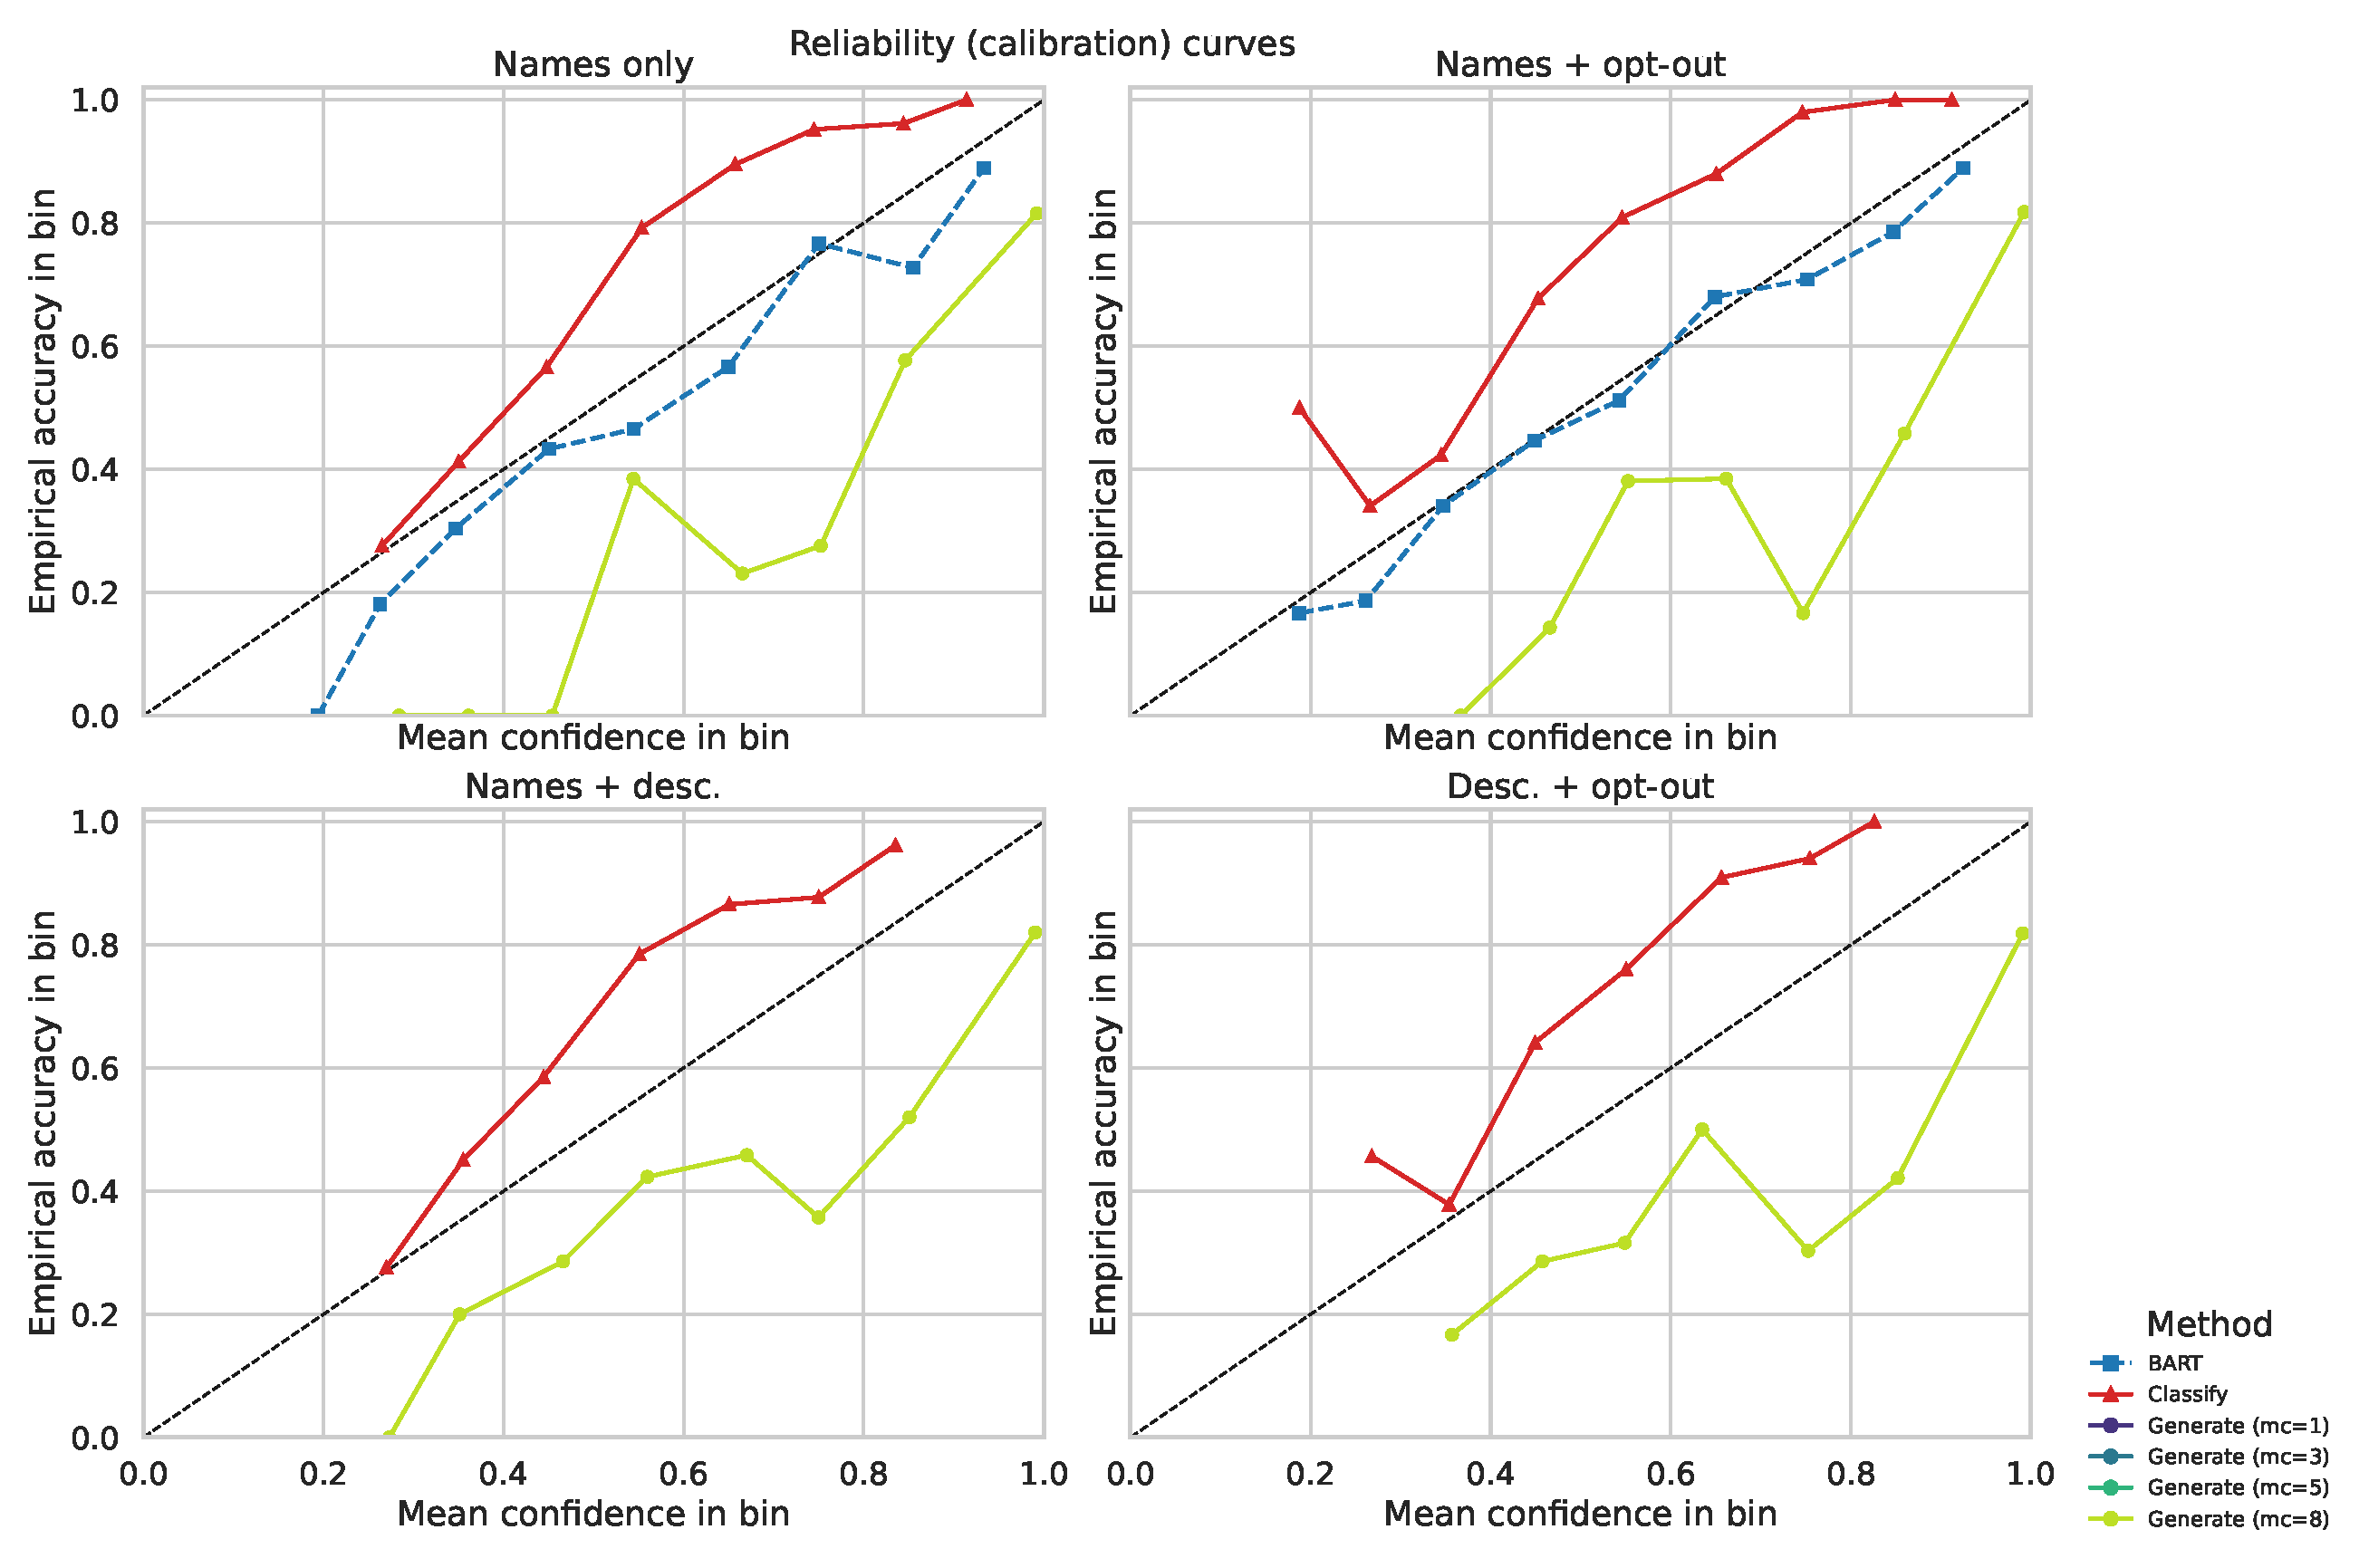
\includegraphics[height=0.65\textheight]{calibration_curve}

  \vspace{0.2em}
  \footnotesize
  BART tracks the diagonal; \texttt{classify} lies \textbf{above} it
  (underconfidence); \texttt{generate} lies \textbf{below} it (overconfidence).
\end{frame}

\begin{frame}{Calibration — Key Finding}
  \begin{itemize}
    \item \textbf{BART} well calibrated (ECE $\approx 0.03$--$0.06$)
    \item \texttt{classify} is \alert{underconfident}: mean confidence $0.59$
          vs.\ accuracy $0.76$; reliability curve above diagonal
    \item \texttt{generate} is \alert{overconfident}: mean confidence $0.94$
          vs.\ accuracy $0.74$; curve below diagonal
    \item Both generative strategies have high ECE ($0.15$--$0.22$) — absolute
          probabilities unreliable
    \item \textbf{But} ranking quality is strong: ROC-AUC of confidence $0.70$
          (BART) vs.\ $0.79$--$0.83$ (\texttt{classify})
  \end{itemize}

  \vspace{0.3em}
  $\to$ Practical deployment: prefer \textbf{ranking-based triage} or
  post-hoc calibration (sharpen \texttt{classify}, soften \texttt{generate}).
\end{frame}

\begin{frame}{Confidence Discrimination — Boxplots}
  \centering
  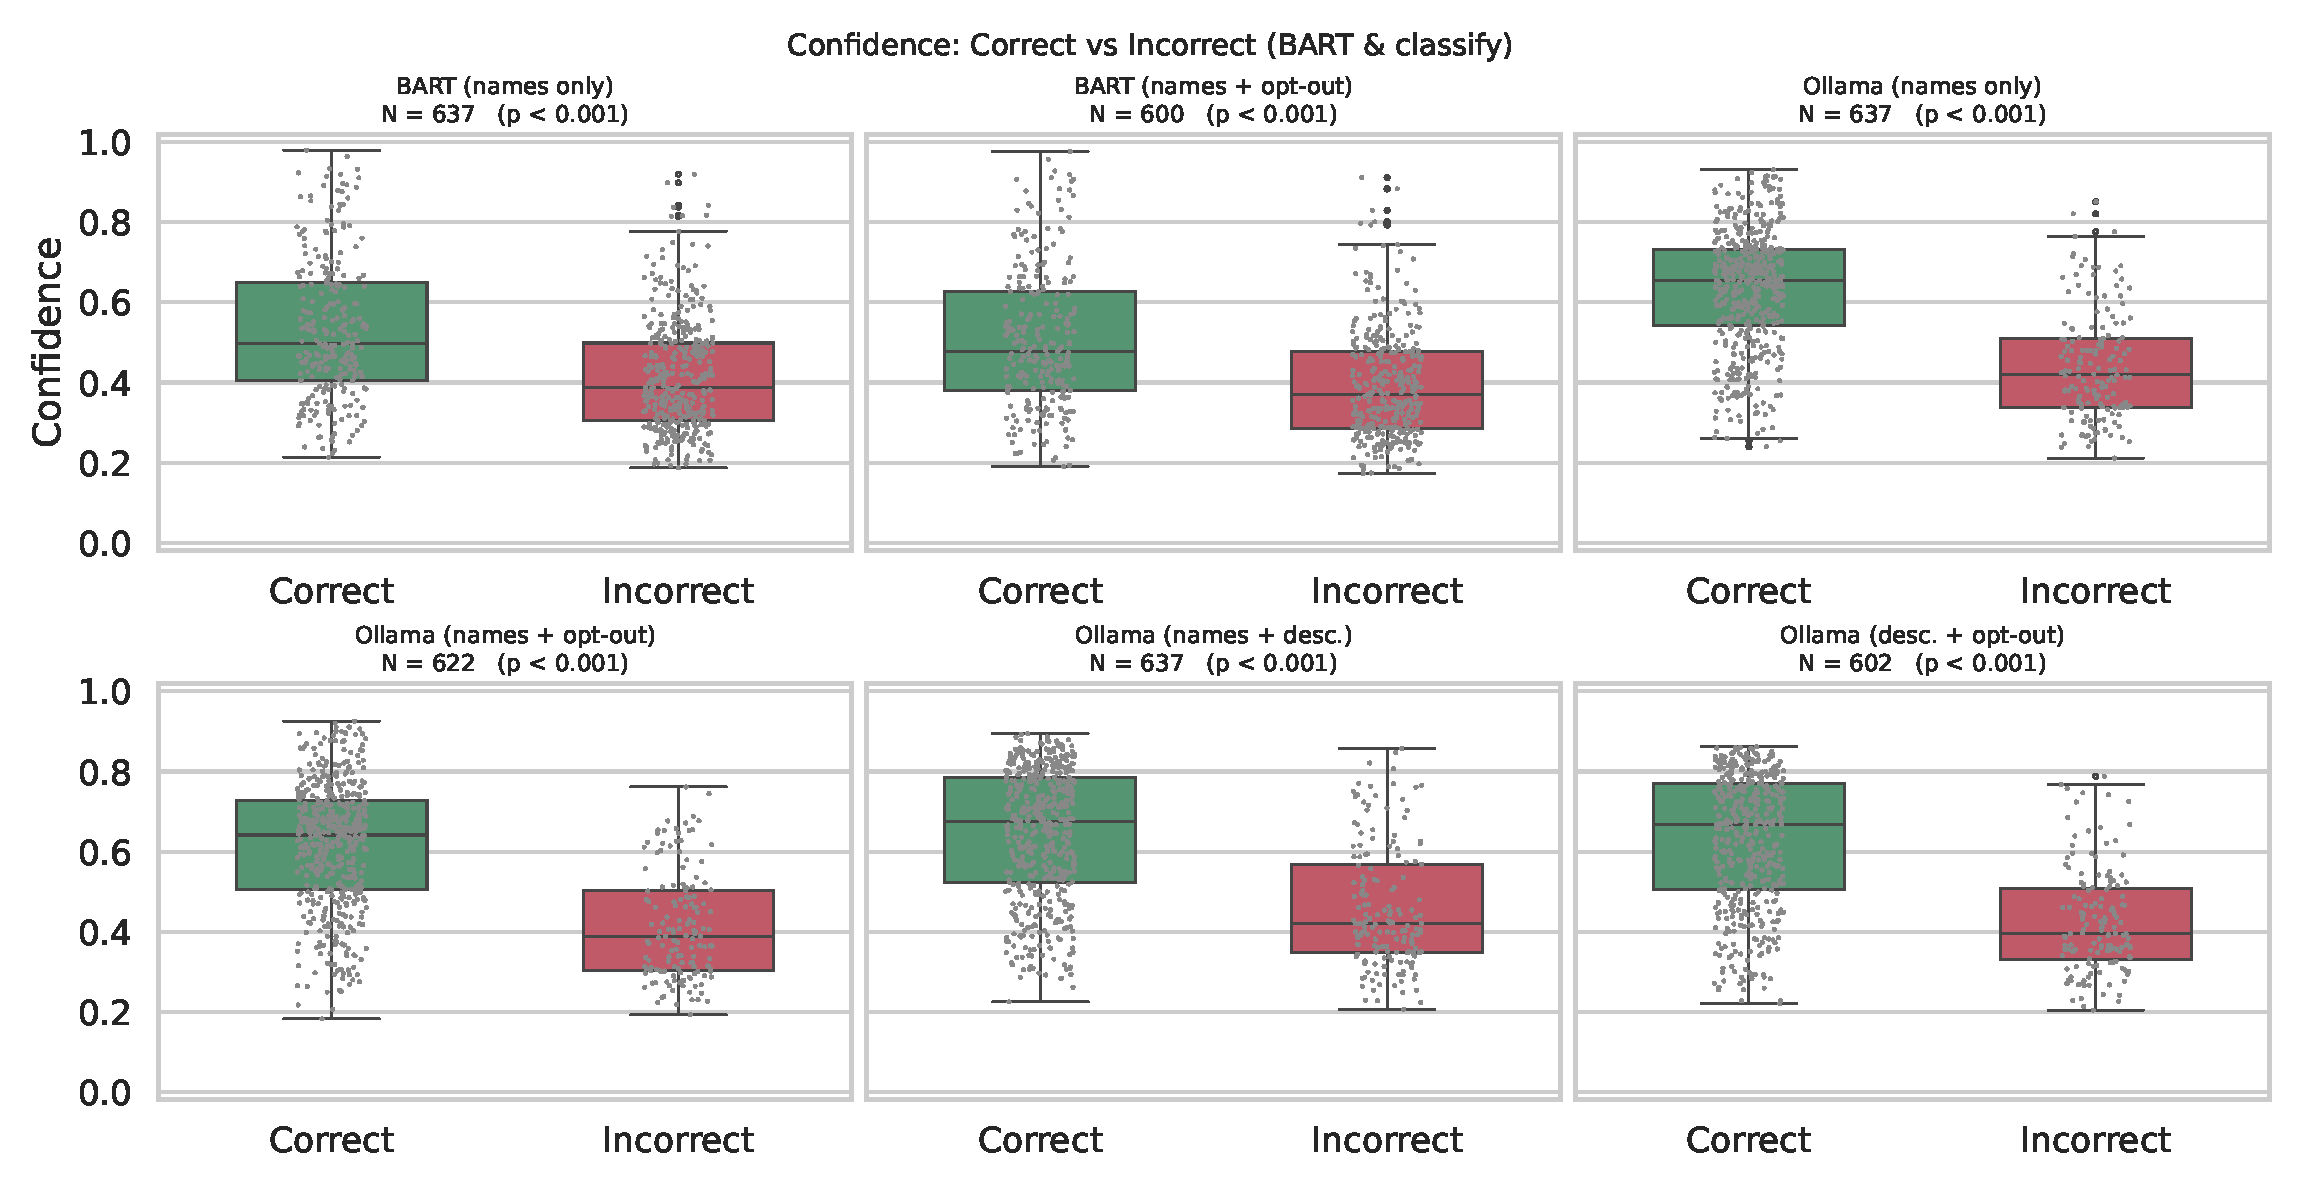
\includegraphics[height=0.72\textheight]{confidence_boxplots_subset}

  \vspace{0.2em}
  \footnotesize
  Welch $t$-tests (correct $>$ incorrect) highly significant ($p<0.001$) for
  all variations.
\end{frame}

\begin{frame}{Score-Gap Discrimination — Boxplots}
  \centering
  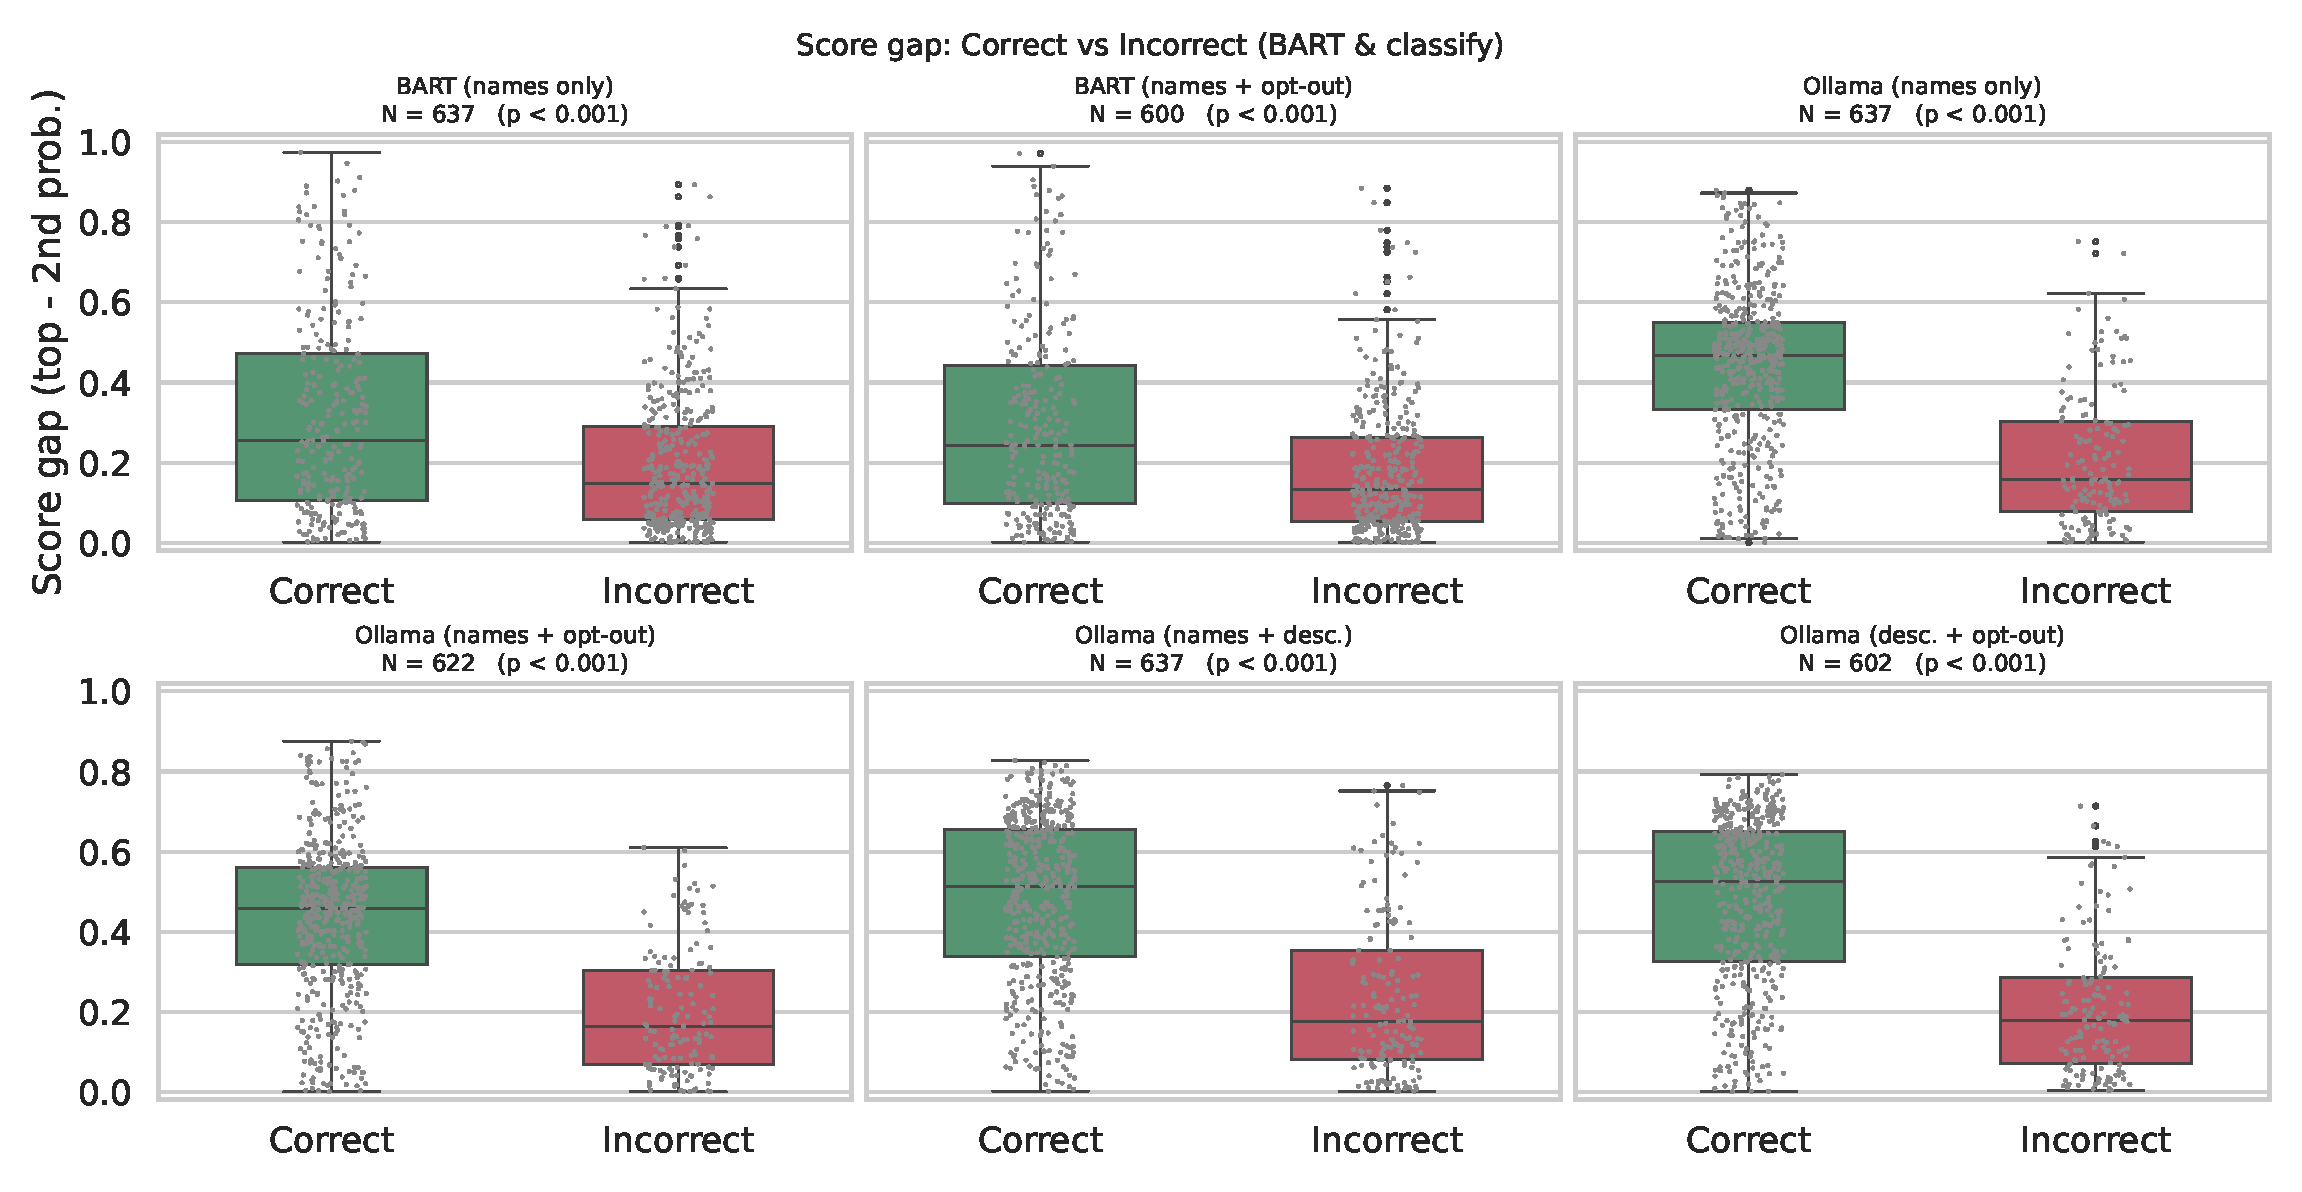
\includegraphics[height=0.72\textheight]{scoregap_boxplots_subset}

  \vspace{0.2em}
  \footnotesize
  The score gap discriminates correctness comparably to confidence.
\end{frame}

\begin{frame}{Confidence \& Calibration Metrics (excerpt)}
  \centering
  \footnotesize
  \resizebox{\textwidth}{!}{%
  \begin{tabular}{lcccccc}
    \toprule
    \textbf{Variation} & \textbf{Conf.\ (corr.)} & \textbf{Conf.\ (inc.)} &
    $\boldsymbol{r}$ & \textbf{ECE} & \textbf{AUC (conf.)} & \textbf{Brier} \\
    \midrule
    BART (names only)          & 0.532 & 0.414 & 0.347 & 0.055 & 0.697 & 0.215 \\
    BART (names + opt-out)     & 0.509 & 0.392 & 0.351 & 0.028 & 0.700 & 0.214 \\
    \addlinespace
    \texttt{classify} (names only)       & 0.632 & 0.442 & 0.488 & 0.170 & 0.820 & 0.171 \\
    \texttt{classify} (names + opt-out)  & 0.617 & 0.413 & 0.493 & 0.196 & 0.831 & 0.176 \\
    \texttt{classify} (names + desc.)    & 0.642 & 0.460 & 0.445 & 0.149 & 0.788 & 0.175 \\
    \texttt{classify} (desc. + opt-out)  & 0.627 & 0.425 & 0.484 & 0.177 & 0.821 & 0.174 \\
    \bottomrule
  \end{tabular}}

  \vspace{0.5em}
  \normalsize
  All Welch $t$-tests significant ($p<0.001$ after BH correction).
  \texttt{classify} has higher AUC but higher ECE than BART.
\end{frame}

\begin{frame}{Threshold-Based Discrimination}
  \centering
  \begin{columns}[T]
    \begin{column}{0.49\textwidth}
      \centering
      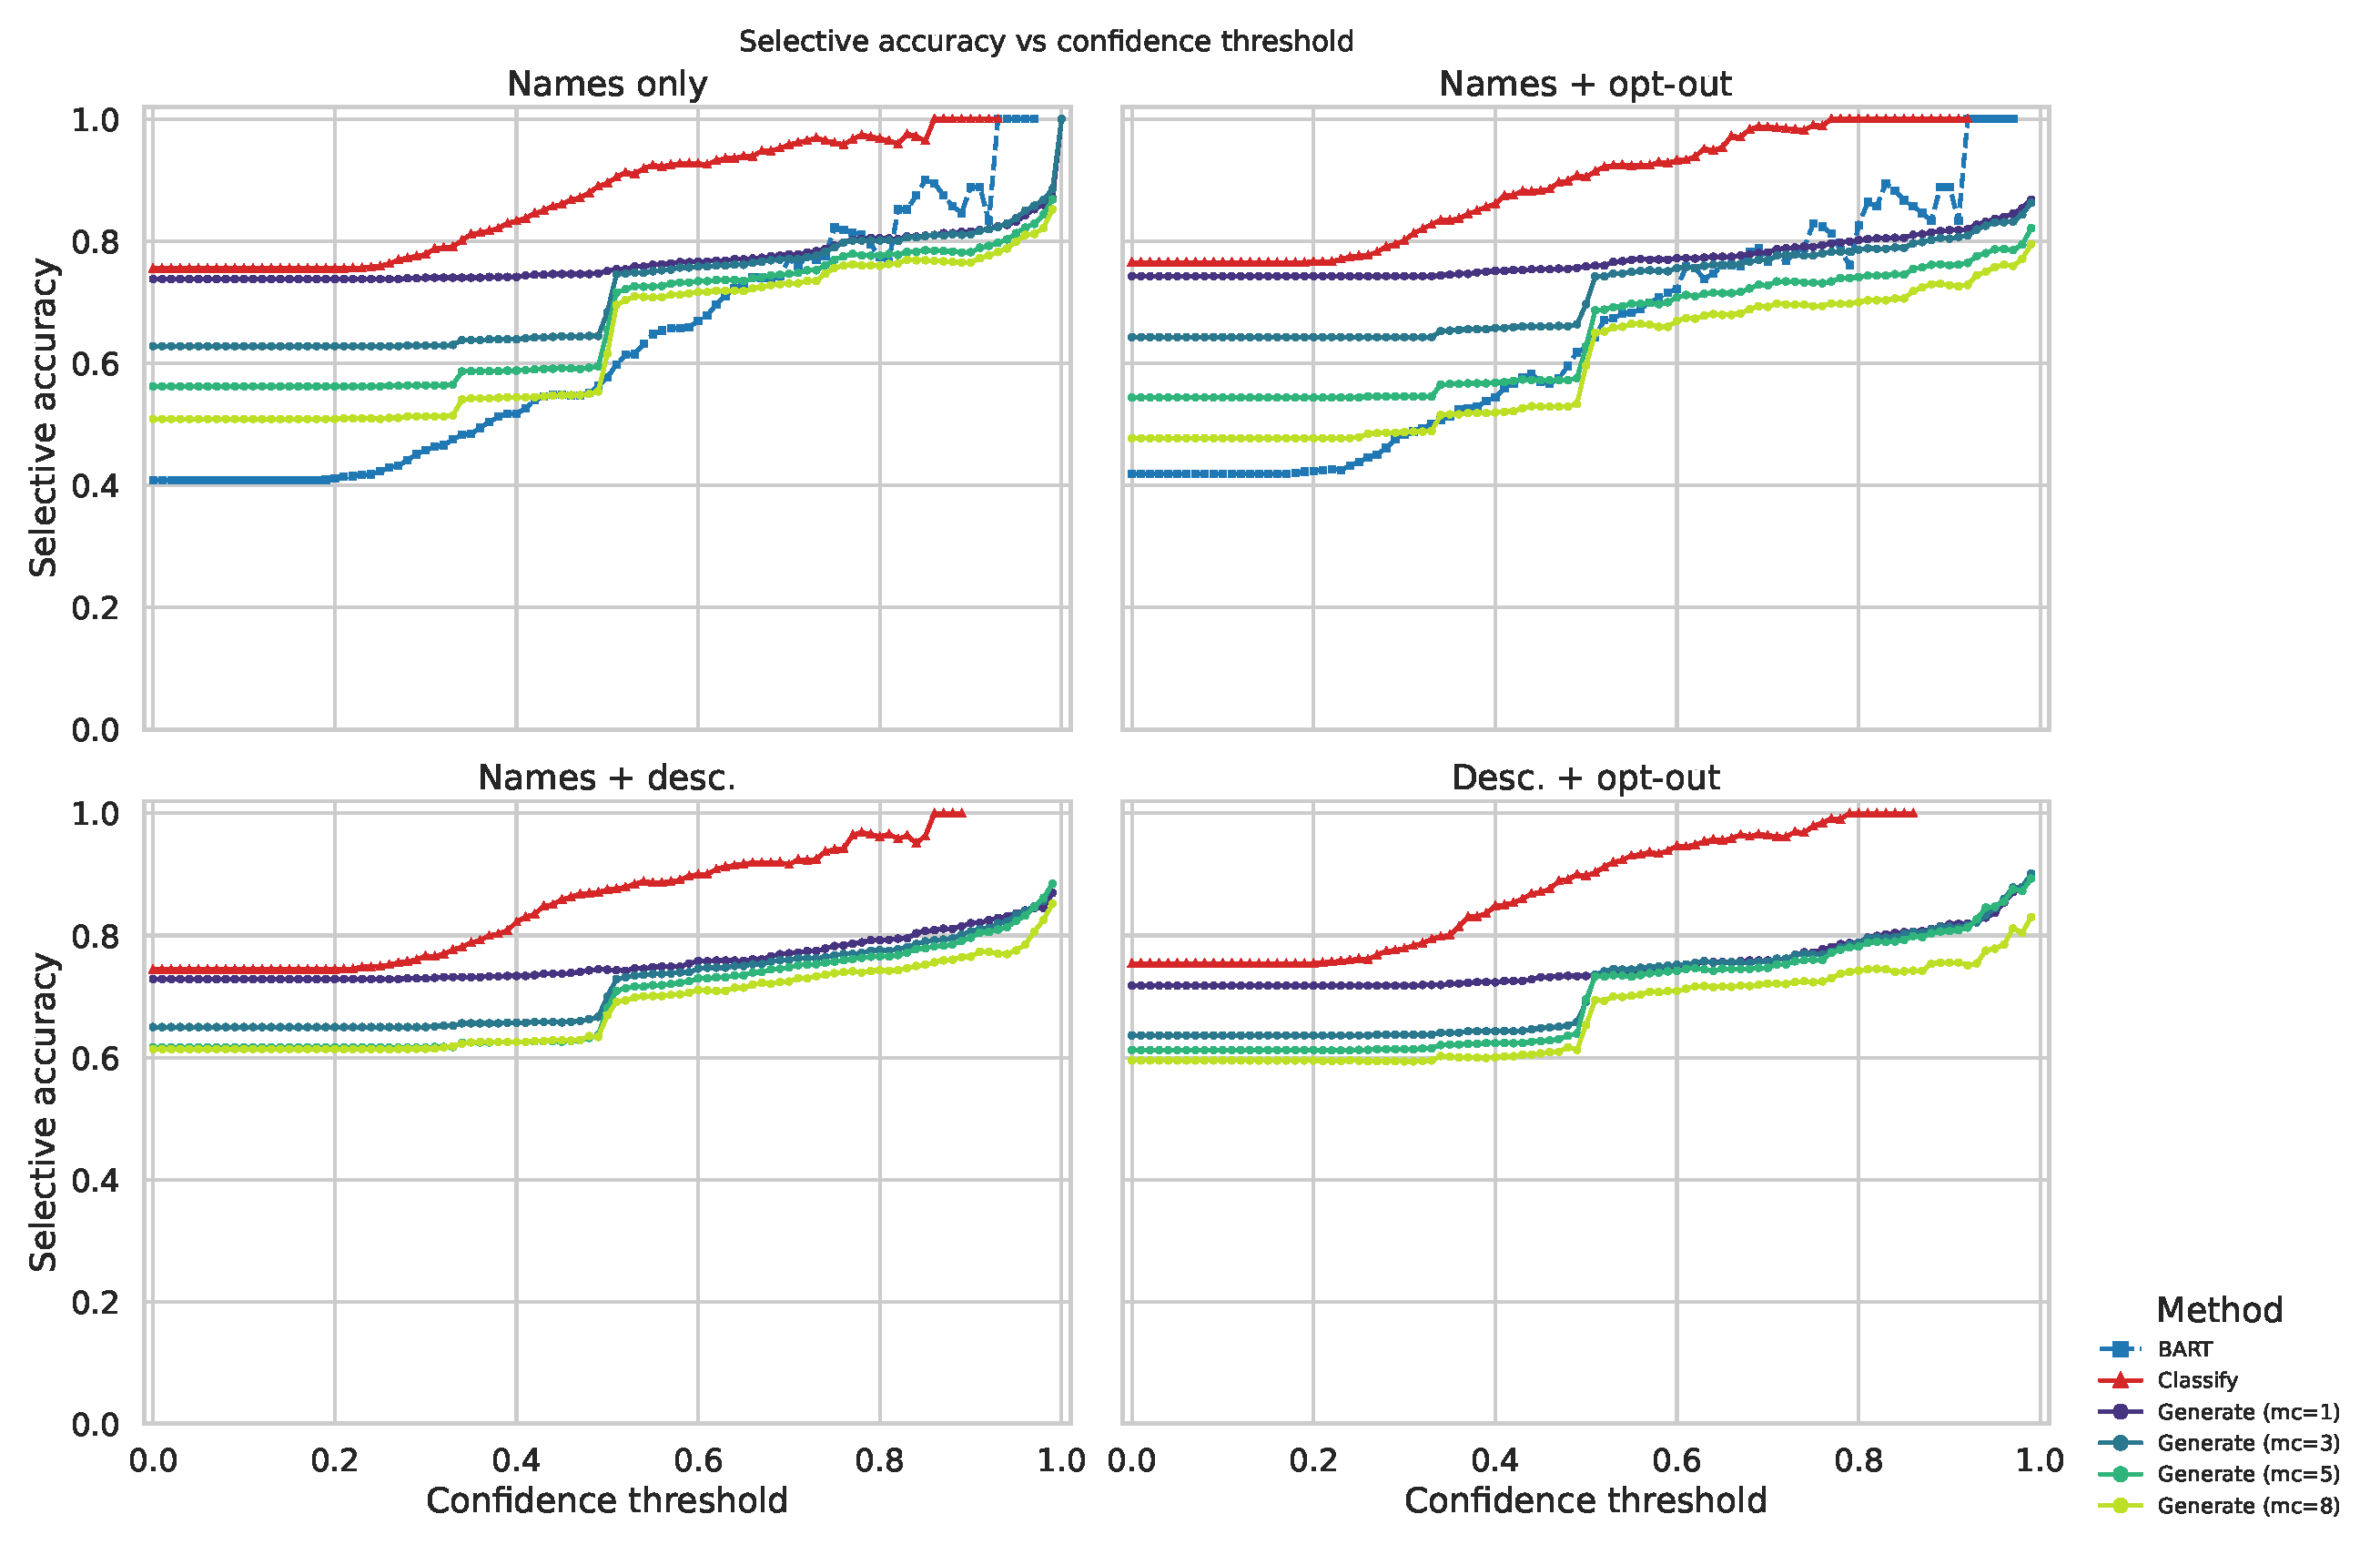
\includegraphics[width=\textwidth]{selective_accuracy}\\
      {\footnotesize Selective accuracy vs.\ confidence threshold}
    \end{column}
    \begin{column}{0.49\textwidth}
      \centering
      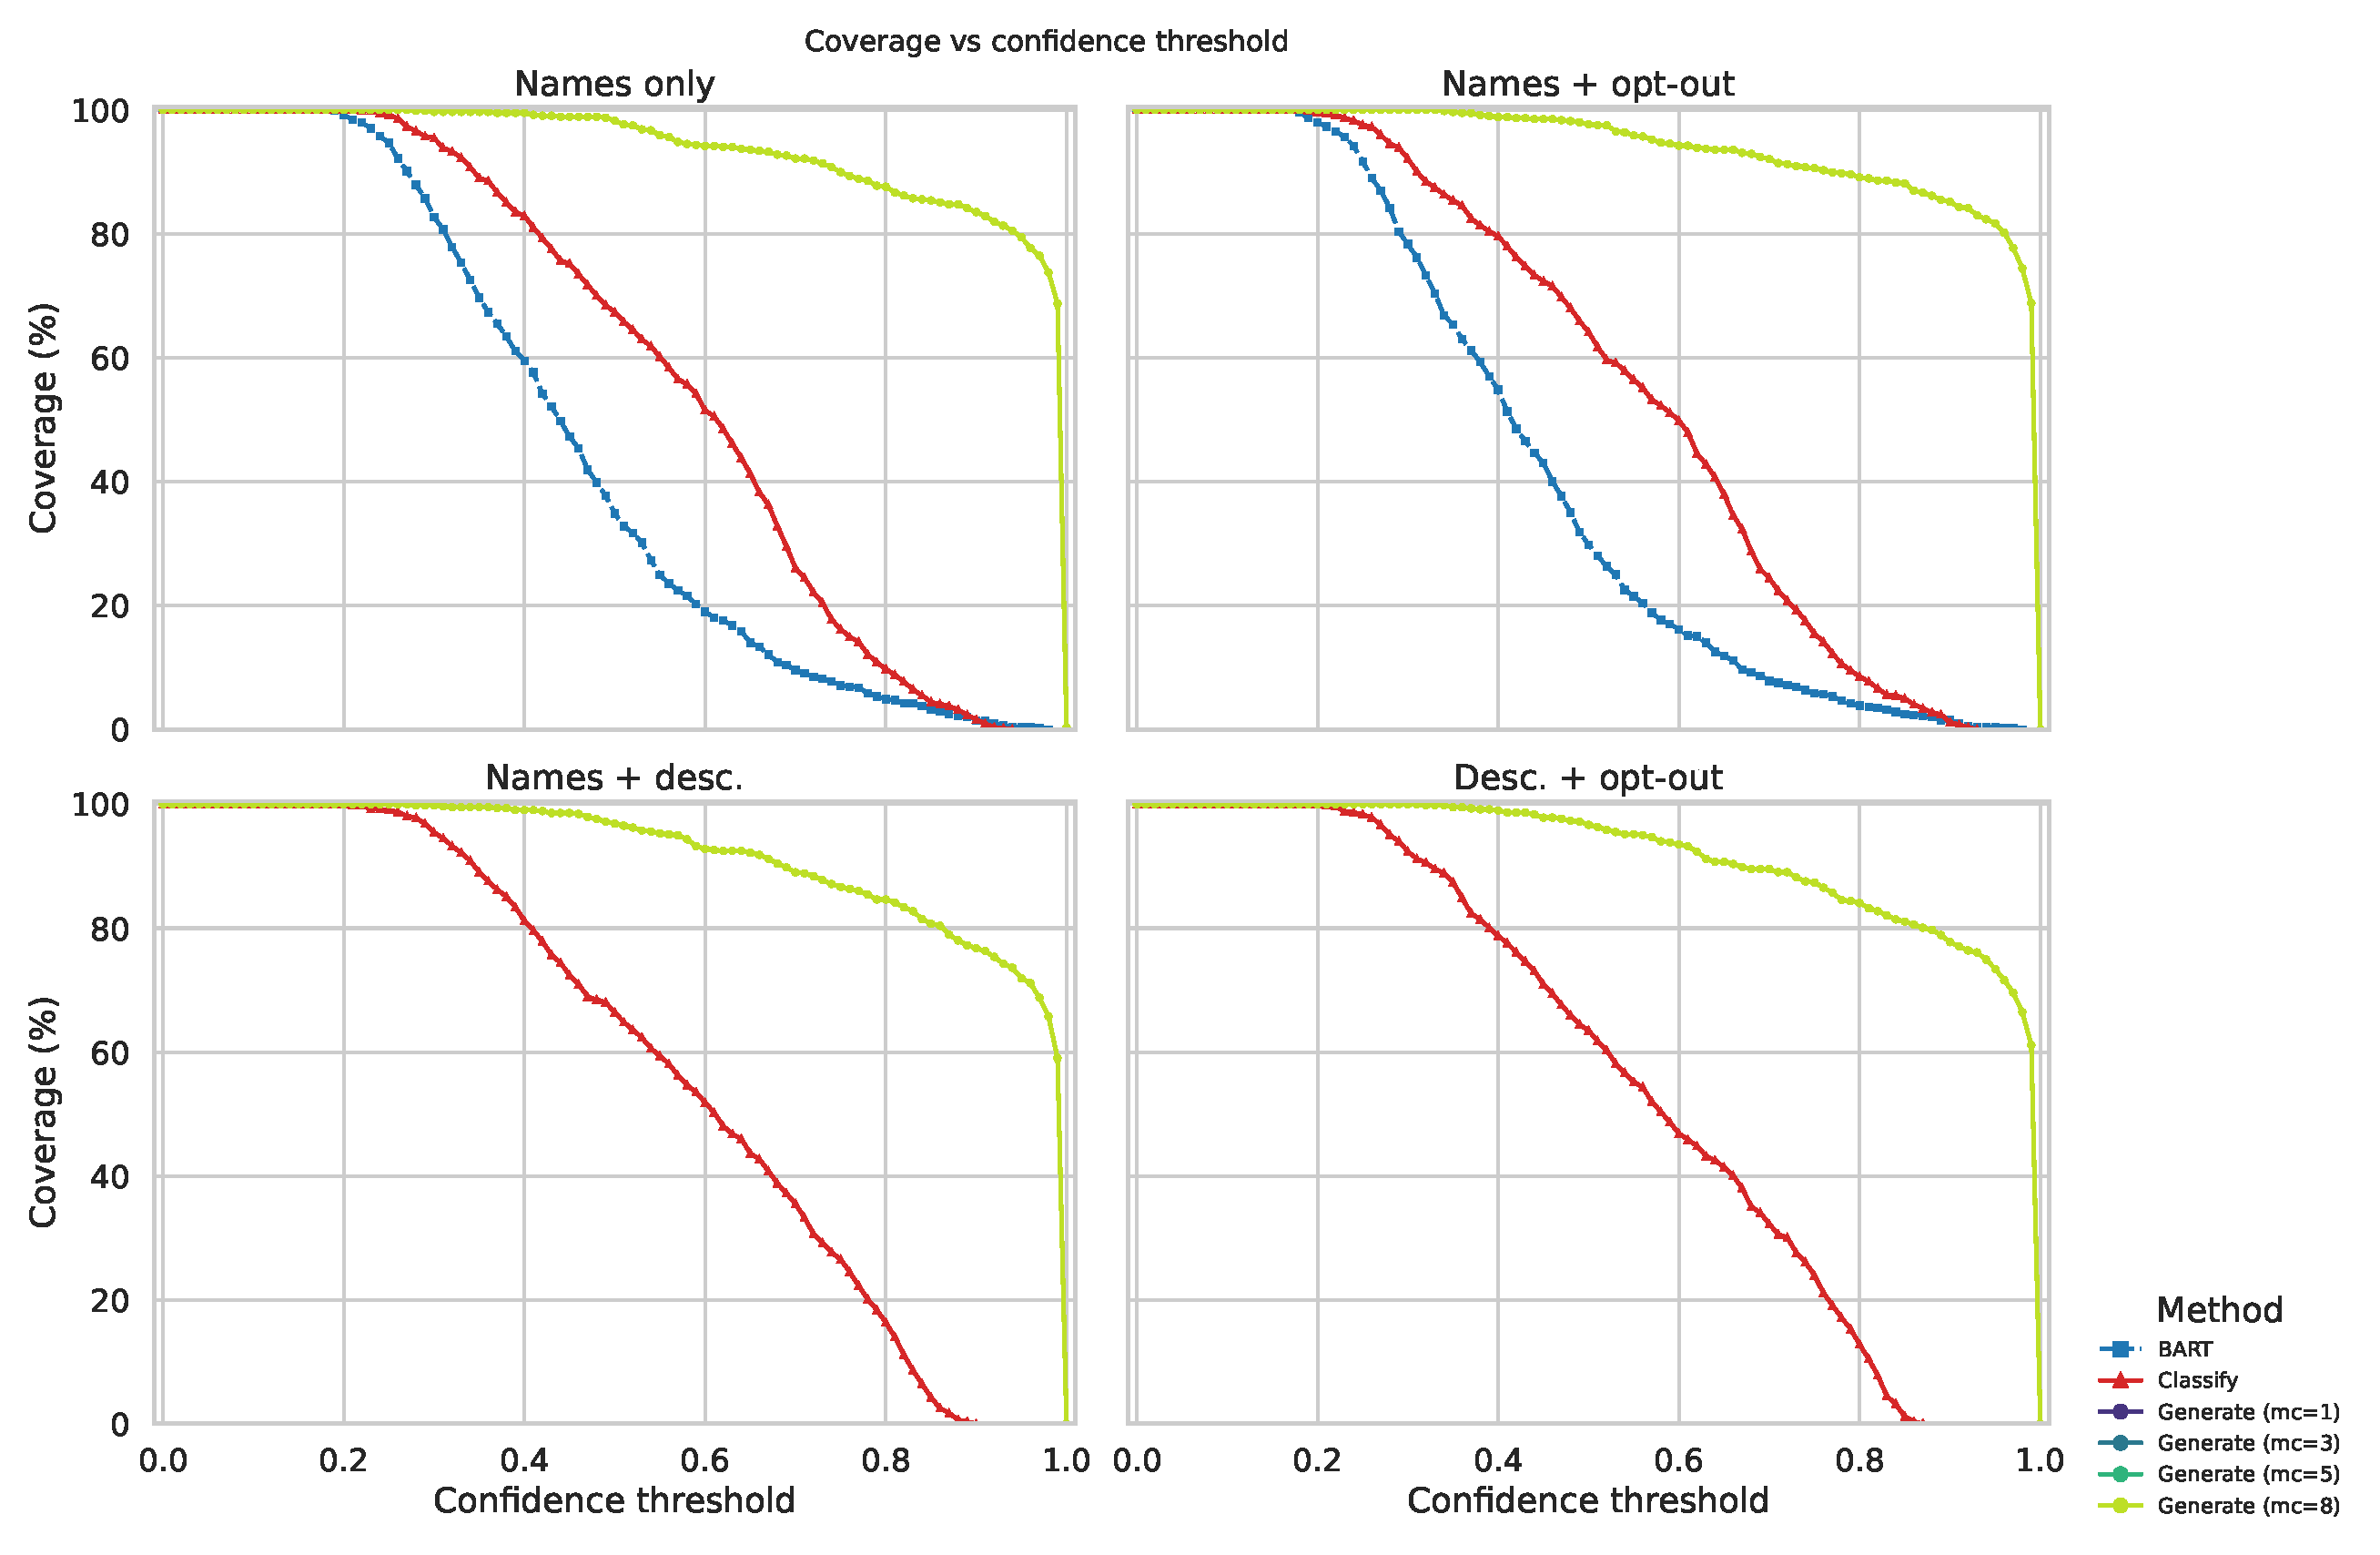
\includegraphics[width=\textwidth]{coverage_curve}\\
      {\footnotesize Coverage vs.\ confidence threshold}
    \end{column}
  \end{columns}

  \vspace{0.4em}
  \normalsize
  Abstaining below the Youden-optimal margin lifts \texttt{classify} accuracy
  from $75.5\% \to 92.8\%$ at $58.6\%$ coverage.
\end{frame}

\begin{frame}{Threshold Discrimination Metrics}
  \centering
  \footnotesize
  \resizebox{\textwidth}{!}{%
  \begin{tabular}{lccccccccc}
    \toprule
    & \multicolumn{4}{c}{\textbf{Confidence threshold}} &
    \multicolumn{4}{c}{\textbf{Margin (score-gap) threshold}} \\
    \cmidrule(lr){2-5}\cmidrule(lr){6-9}
    \textbf{Variation} & \textbf{AUC} & \textbf{thr.} & \textbf{sel.\ acc.} & \textbf{cov.}
    & \textbf{AUC} & \textbf{thr.} & \textbf{sel.\ acc.} & \textbf{cov.} \\
    & & & (\%) & (\%) & & & (\%) & (\%) \\
    \midrule
    BART (names only)       & 0.697 & 0.42 & 54.4 & 53.4 & 0.640 & 0.34 & 60.9 & 27.3 \\
    BART (+ opt-out)        & 0.700 & 0.41 & 56.3 & 51.8 & 0.644 & 0.27 & 59.5 & 33.3 \\
    \addlinespace
    \texttt{classify} (names only)       & 0.820 & 0.52 & 91.3 & 64.7 & 0.809 & 0.36 & 92.8 & 58.6 \\
    \texttt{classify} (+ opt-out)        & 0.831 & 0.53 & 92.4 & 59.3 & 0.817 & 0.34 & 93.0 & 60.0 \\
    \texttt{classify} (+ desc.)          & 0.788 & 0.54 & 89.0 & 61.2 & 0.799 & 0.30 & 89.0 & 65.6 \\
    \texttt{classify} (desc. + opt-out)  & 0.821 & 0.55 & 93.4 & 55.0 & 0.831 & 0.32 & 91.8 & 62.6 \\
    \bottomrule
  \end{tabular}}

  \vspace{0.4em}
  \normalsize
  The score gap is as informative as confidence — sometimes more (desc.\ +
  opt-out: AUC $0.831$ vs.\ $0.821$).
\end{frame}

\begin{frame}{Adaptive \texttt{generate} Strategy}
  \centering
  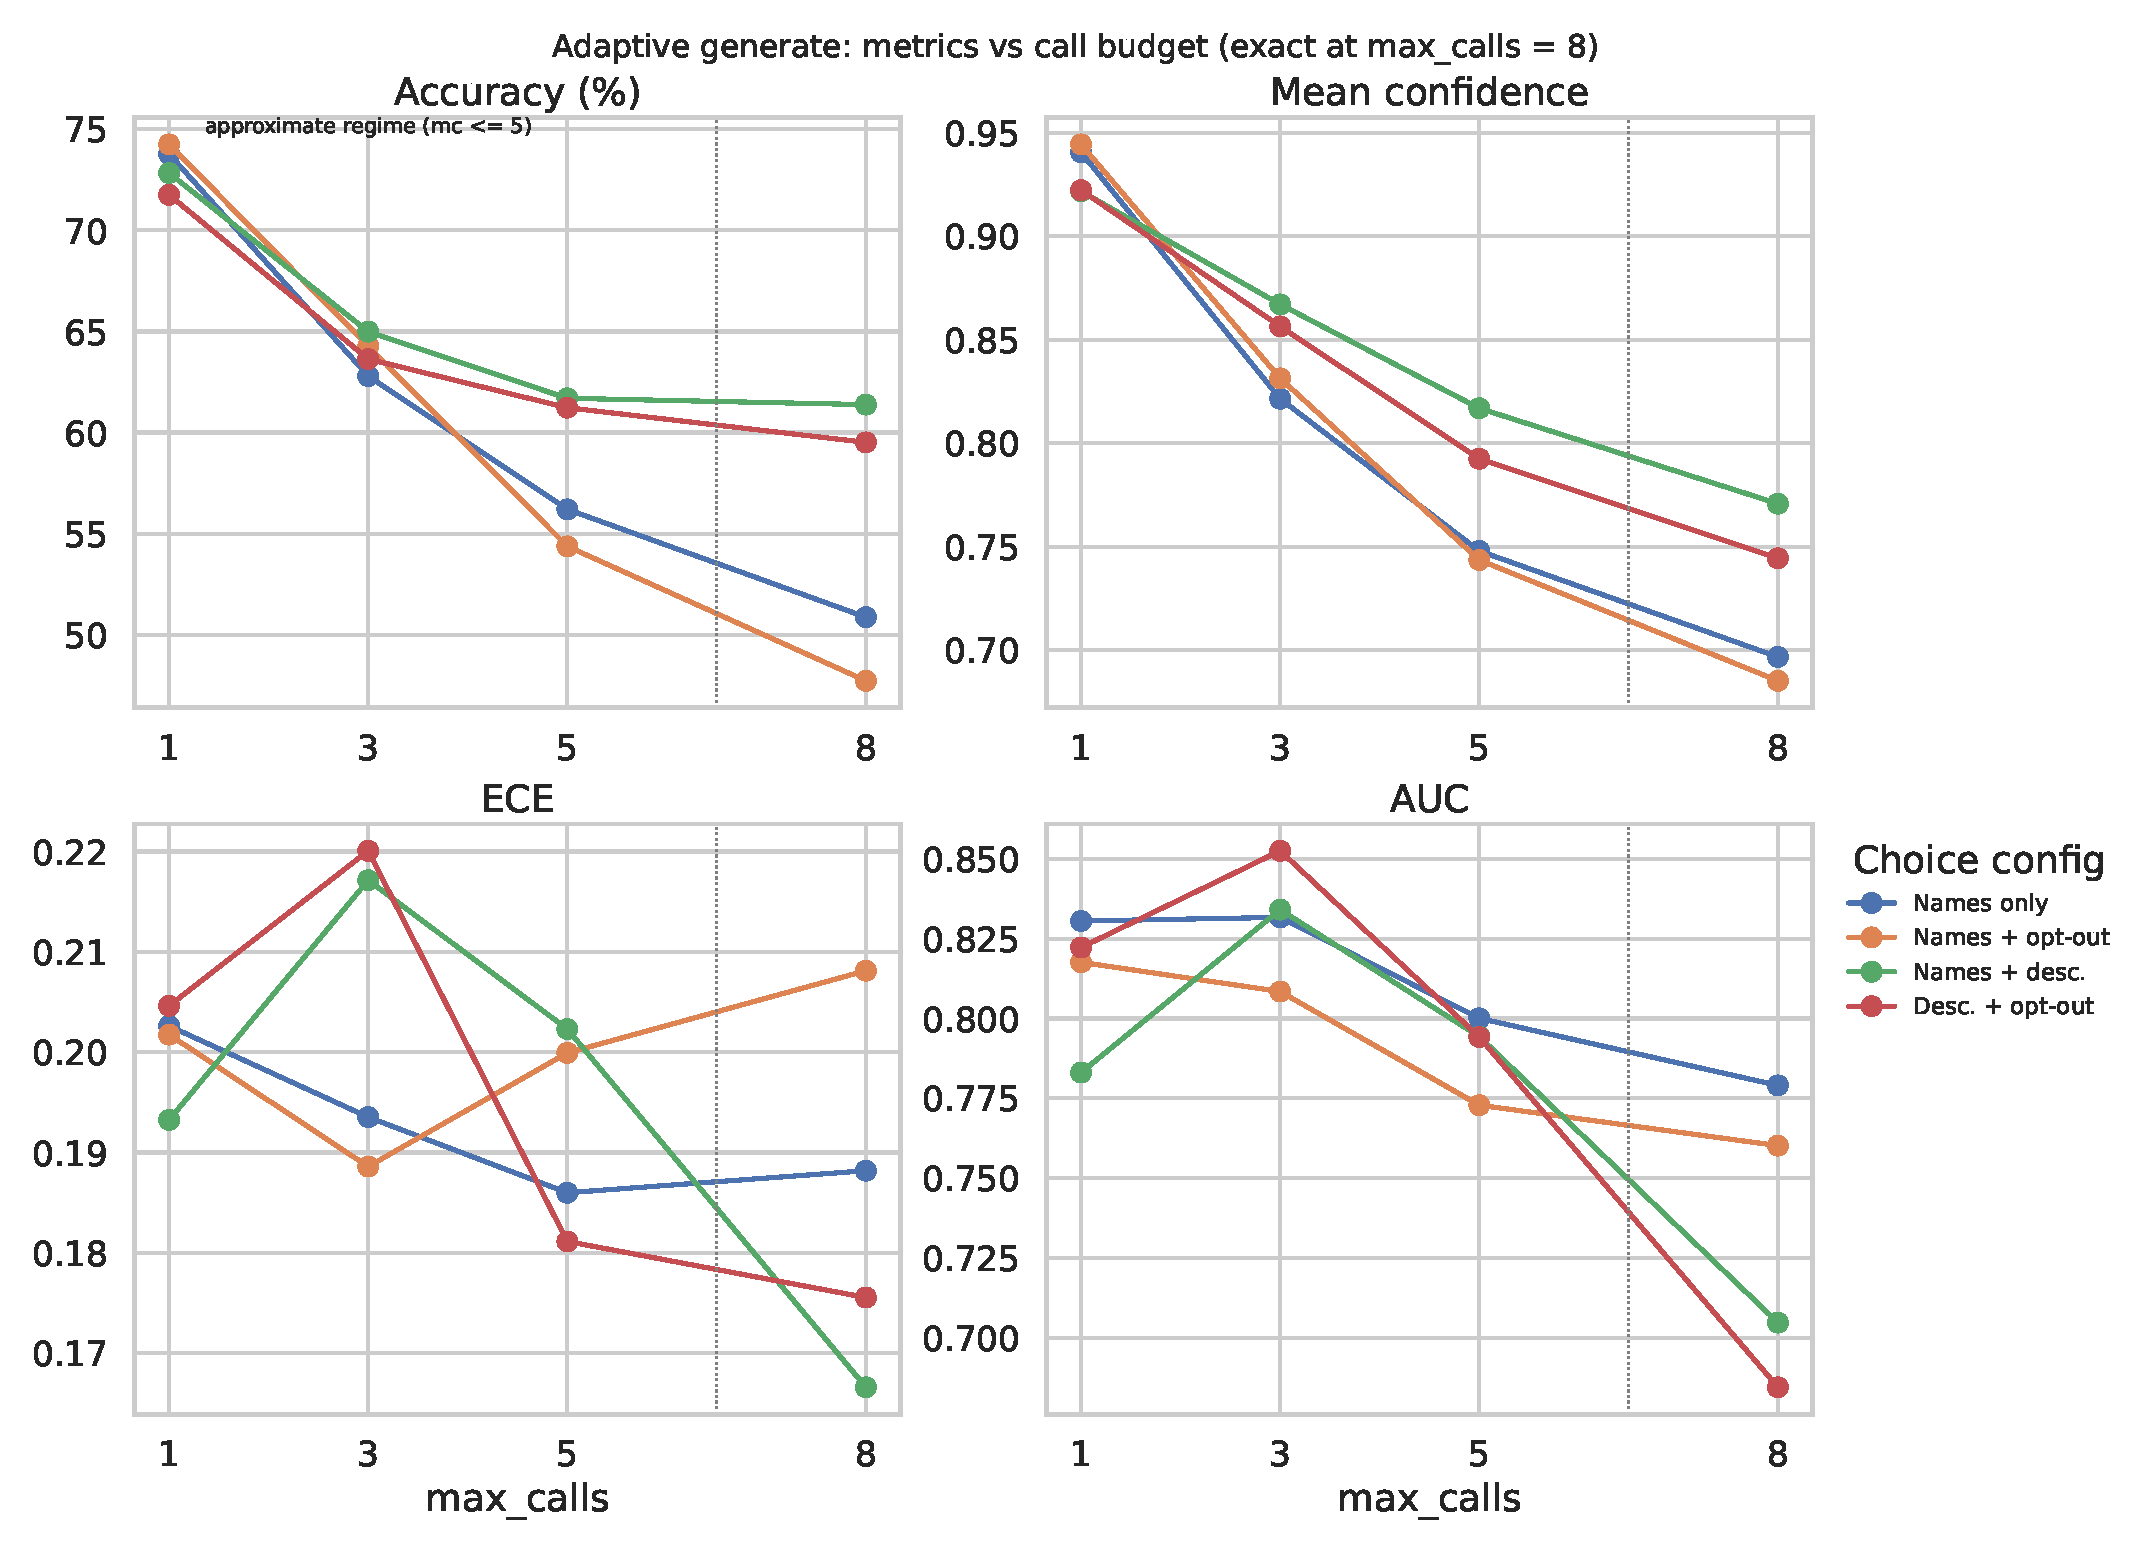
\includegraphics[height=0.72\textheight]{generate_sweep}

  \vspace{0.2em}
  \footnotesize
  At \texttt{max\_calls}$=1$, \texttt{generate} matches scikit-llm ($73.8\%$);
  accuracy falls monotonically as budget grows.
\end{frame}

% =============================================================================
\section{Discussion \& Conclusion}
% =============================================================================

\begin{frame}{Design Decisions}
  \begin{enumerate}
    \item \textbf{Local-first:} Ollama by default; vLLM, SGLang, llama.cpp
          for matching hardware
    \item \textbf{No fine-tuning:} prompting + retrieval $\to$ maximum
          flexibility, no retraining
    \item \textbf{Two scoring strategies} with explicit cost--accuracy
          trade-off:
          \begin{itemize}
            \item \texttt{classify}: one call per label, exact probabilities
            \item \texttt{generate}: budget-controlled, flags approximate
                  results via coverage field
          \end{itemize}
  \end{enumerate}
\end{frame}

\begin{frame}{Limitations}
  \begin{itemize}
    \item Classification quality depends on underlying model ($\geq 3$B
          parameters recommended)
    \item LLM-based classification subject to \textbf{data-driven bias} —
          audit in sensitive settings
    \item Multi-call \texttt{classify} expensive for very large label sets
          $\to$ \texttt{generate} preferable
    \item Generative strategies \textbf{miscalibrated} (opposite directions)
          $\to$ use ranking-based triage or post-hoc calibration
    \item GUI is single-user desktop; multi-user server deployment left to
          future work
  \end{itemize}
\end{frame}

\begin{frame}{Conclusion}
  \begin{itemize}
    \item \textbf{\texttt{ollama-classifier}}: open-source Python library for
          zero-shot classification with locally-hosted LLMs
    \item Two confidence-bearing strategies across \textbf{four inference
          backends}
    \item Desktop GUI + cross-language ports (R, Rust)
    \item Compact 3B model \textbf{substantially outperforms BART} NLI
          baseline and \textbf{matches scikit-llm}
    \item Confidence scores and score gaps \textbf{reliably discriminate}
          correct from incorrect predictions
    \item Support effective \textbf{threshold-based triage}
          ($75.5\% \to 92.8\%$ at $58.6\%$ coverage)
  \end{itemize}

\end{frame}

\begin{frame}[standout]
  Thank You
\end{frame}

\begin{frame}{Links \& Contact}
  \textbf{Links:}
  \begin{itemize}
    \item \texttt{ollama-classifier}: \texttt{pip install ollama-classifier}
    \item \texttt{ollama-classifier-gui}: \texttt{uvx ollama-classifier-gui}
    \item \texttt{rollama-classifier}:
          \texttt{pak::pak("paluigi/rollama-classifier")}
    \item \texttt{ollama-classifier-rs}: \texttt{ollama-classifier-rs = "0.5"}
  \end{itemize}

  \vspace{0.5em}
  \textbf{Contact:}\\
  Luigi Palumbo - luigi.palumbo@bancaditalia.it \\
  Mengting Yu - mengting.yu@unitus.it
\end{frame}

\end{document}
